\documentclass[11pt,letterpaper,titlepage]{article}
\usepackage{fancyhdr}
\usepackage[left=0.75in, right=0.75in, bottom=1.0in]{geometry}
\usepackage{lastpage}
\usepackage{titleref}
\usepackage{booktabs}
\usepackage{appendix}
\appendixtitleon
\appendixtitletocon

\makeatletter

%================== List of figures and tables mods
\usepackage{tocloft}
\usepackage[labelfont=bf]{caption}

\renewcommand{\cftfigpresnum}{Figure\ }
\renewcommand{\cfttabpresnum}{Table\ }

\newlength{\mylenf}
\settowidth{\mylenf}{\cftfigpresnum}
\setlength{\cftfignumwidth}{\dimexpr\mylenf+1.5em}
\setlength{\cfttabnumwidth}{\dimexpr\mylenf+1.5em}


\newcommand{\half}{\frac{1}{2}}


%=================== Graphics
\usepackage{graphicx}
\usepackage[breakwords]{truncate}
\usepackage{float}
\usepackage{array}
\usepackage{amsmath}
\usepackage{mdframed}
\usepackage{fancyvrb}
\usepackage{float}
\usepackage{cancel}
\usepackage{amssymb}
\graphicspath{ {images/} }
\usepackage[usenames,dvipsnames,svgnames,table]{xcolor}
\usepackage[defaultlines=2,all]{nowidow}
\usepackage{listings}
\usepackage{color}
\definecolor{Brown}{cmyk}{0,0.81,1,0.60}
\definecolor{OliveGreen}{cmyk}{0.64,0,0.95,0.40}
\definecolor{CadetBlue}{cmyk}{0.62,0.57,0.23,0}
\usepackage{pdflscape}
\usepackage{relsize}
\usepackage{verbatim}
\usepackage{tabto}
%\usepackage{minted}

\lstdefinestyle{myLuastyle}
{
  language         = {[5.0]Lua},
  basicstyle       = \ttfamily,
  showstringspaces = false,
  upquote          = true,
}


%=================== Settings
\renewcommand{\baselinestretch}{1.2}
\definecolor{gray}{rgb}{0.4 0.4 0.4}
\newcommand{\stimes}{{\times}}

\begin{document}
\newcommand{\NSCDOCNUMBR}{NSC-REP-15-X}         %Put document number here
\newcommand{\NSCDOCSUBJT}{TECHNICAL REPORT: }   %Put document subject here
\newcommand{\NSCDOCTITLE}{$THERMOALPHA-Heatblock$ - Input Manual}       %Put document title here
\newcommand{\NSCDOCDATE} {February, 2017}    %Put document date here
\newcommand{\NSCDOCREV}  {Rev 1.0} %Put revision number here

\lstset{language=C++,frame=ltrb,framesep=4pt,basicstyle=\linespread{0.8} \small,
	keywordstyle=\ttfamily\color{OliveGreen},
	identifierstyle=\ttfamily\color{CadetBlue}\bfseries,
	commentstyle=\color{Brown},
	stringstyle=\ttfamily,
	showstringspaces=ture }


%################################# TITLE PAGE ########################
\begin{titlepage}
	\pagestyle{fancy}
	\vspace*{1.0cm}
	\centering
	%\includegraphics{NSC_Logo} \par
	\vspace{1cm}
	%\centering
	%{\Large\bfseries  \NSCDOCNUMBR   \par}
	\vspace{.25cm}
	%\centering
	{\Large\bfseries  \NSCDOCSUBJT \par} 
	{\Large\bfseries \NSCDOCTITLE  \par}
	\vspace{1cm}
	{\Large \NSCDOCDATE \par}
	\vspace{1.0cm}
	{\Large Jan Vermaak \par}
	{\Large \NSCDOCREV \par}
		
	\begin{comment}
	\renewcommand{\arraystretch}{2.0}
	\begin{tabular}{| m{2.5cm} | m{4.5cm} | m{4.5cm} |}
		\cline{2-3}
		\multicolumn{1}{c|}{} & \bfseries{Name} & \bfseries{Signature \& Date} \\ \hline
		\bfseries{Prepared} &     &     \\ \hline
		\bfseries{Reviewed} &     &     \\ \hline
		\bfseries{Reviewed} &     &     \\ \hline
	    \bfseries{Approved} &     &     \\ \hline
	\end{tabular} \par
	\end{comment}
	\begin{center}
		\begin{minipage}[c]{0.45\textwidth}
			\begin{figure}[H]
			
				
\includegraphics[width=3in]{Logo2_Medium.png}
			\end{figure}
		\end{minipage}
	\end{center}
	\vspace{2cm}
	%NSC-FRM-15-1 Rev.1
\end{titlepage}


\pagestyle{fancy}
\rfoot{Page \thepage \ of \pageref{LastPage}}
%\cfoot{NSC-FRM-15-1 Rev.1}
\cfoot{}
\lfoot{\truncate{14cm}{\NSCDOCTITLE}}
\rhead{}
\chead{\currentname}
\lhead{}
\renewcommand{\footrulewidth}{0.4pt}
\tableofcontents
\addtocontents{toc}{~\hfill\textbf{Page}\par}

\listoffigures
%\listoftables
\chead{Contents}


\newpage
\chead{1 The Input File}
\section{The Input File}
The initial simulation setup of a radial heat conduction model is performed using an input file. The input file specifies all the parameters needed to define a heatblock as shown in Figure \ref{figure:ZZZ_HeatBlock} below. Physical regions are contained in \textbf{intervals} and temperatures are calculated at \textbf{nodes}. The simulation is one-dimensional (1D) and therefore does not account for azimuthal- or axial heat conduction.

	\begin{center}
		\begin{minipage}[c]{0.85\textwidth}
	
			\begin{figure}[H]
			
				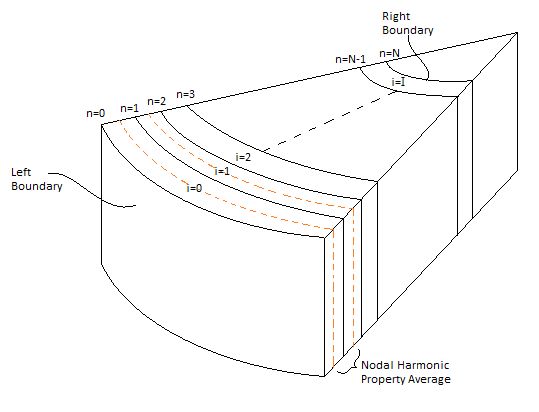
\includegraphics[width=6in]{ZZZ_HeatBlock.png}
				\caption{Heat block nodalization.}
				\label{figure:ZZZ_HeatBlock}
			\end{figure}
		\end{minipage}
	\end{center}
\vspace{0.5cm}
\newpage
\noindent
The $Heatblock$ input cards are entered on the same file used for the input to $Thermoalpha$. The input cards include:
\begin{itemize}
\item \textbf{HEATBLOCK}, defines the mesh.
\item \textbf{HEATBLOCKK}, defines interval thermal conductivity $k$.
\item \textbf{HEATBLOCKC}, defines interval heat capacity $C_p$.
\item \textbf{HEATBLOCKRHO}, defines interval density $\rho$.
\item \textbf{HEATBLOCKT}, defines initial nodal temperature $T_n$.
\item \textbf{HEATBLOCKL}, defines left boundary condition.
\item \textbf{HEATBLOCKR}, defines right boundary condition.
\item \textbf{HEATBLOCKSHAPE}, defines radial heat generation profile.
\item \textbf{HEATBLOCKE}, defines block average heat generation rate.
\end{itemize}




\vspace{0.5cm}
\subsection{HEATBLOCK}
Defines the amount of nodes and radial mesh spacing.
\begin{itemize}
\item \textbf{Word 1}. [String] Heatblock name. Maximum 200 characters.
\item \textbf{Word 2}. [Integer] Number of nodes in the spatial mesh $N$.
\item \textbf{Word 3 to ($3+N$)}. [Float] Nodal radius value. This value cannot be negative. The values of each nodal radius must be monotonically decreasing and will result in a crash if specified otherwise.
\end{itemize}

\vspace{0.5cm}
\subsection{HEATBLOCKK}
Defines interval thermal conductivity $k$.
\begin{itemize}
\item \textbf{Word 1}. [String] Heatblock name. Maximum 200 characters.
\item \textbf{Word 2 to ($2+I$)}. [Float] Interval thermal conductivity $k$.
\end{itemize}

\vspace{0.5cm}
\subsection{HEATBLOCKC}
Defines interval heat capacity $C_p$.
\begin{itemize}
\item \textbf{Word 1}. [String] Heatblock name. Maximum 200 characters.
\item \textbf{Word 2 to ($2+I$)}. [Float] Interval heat capacity $C_p$.
\end{itemize}

\vspace{0.5cm}
\subsection{HEATBLOCKRHO}
Defines interval density $\rho$.
\begin{itemize}
\item \textbf{Word 1}. [String] Heatblock name. Maximum 200 characters.
\item \textbf{Word 2 to ($2+I$)}. [Float] Interval density $\rho$.
\end{itemize}

\vspace{0.5cm}
\subsection{HEATBLOCKT}
Defines initial nodal temperature $T_n$.
\begin{itemize}
\item \textbf{Word 1}. [String] Heatblock name. Maximum 200 characters.
\item \textbf{Word 2 to ($2+N$)}. [Float] Initial nodal temperature $T_n$.
\end{itemize}

\vspace{0.5cm}
\subsection{HEATBLOCKL}
Defines the left boundary condition.
\begin{itemize}
\item \textbf{Word 1}. [String] Heatblock name. Maximum 200 characters.
\item \textbf{Word 2}. [Integer] Boundary condition type. $1$-convection boundary condition, $2$-symmetry/insulated boundary condition, $3$-heat flux. If this word is $1$ then words 3 and 4 are convection coefficient $h$ and bulk coolant temperature $T_b$. If this word is $2$ then words 3 and 4 are ignored. If this word is $3$ then word 3 is the specified heat flux and word 4 is ignored.
\item \textbf{Word 3}. [Float] Required if word 2 is $1$ or $3$. If word 2 is $1$ then this word is the convection coefficient $h$ [$W.m^{-2}.K^{-1}$]. If word 2 is $3$ then this word is the specified heat flux $q''$ [$W.m^{-2}$].
\item \textbf{Word 4}. [Float] Required if word 2 is $1$. This word is the bulk coolant temperature $T_b$ [$C$] associated with the convection coefficient in word 3.
\end{itemize}

\vspace{0.5cm}
\subsection{HEATBLOCKR}
Defines the right boundary condition.
\begin{itemize}
\item \textbf{Word 1}. [String] Heatblock name. Maximum 200 characters.
\item \textbf{Word 2}. [Integer] Boundary condition type. $1$-convection boundary condition, $2$-symmetry/insulated boundary condition, $3$-heat flux. If this word is $1$ then words 3 and 4 are convection coefficient $h$ and bulk coolant temperature $T_b$. If this word is $2$ then words 3 and 4 are ignored. If this word is $3$ then word 3 is the specified heat flux and word 4 is ignored.
\item \textbf{Word 3}. [Float] Required if word 2 is $1$ or $3$. If word 2 is $1$ then this word is the convection coefficient $h$ [$W.m^{-2}.K^{-1}$]. If word 2 is $3$ then this word is the specified heat flux $q''$ [$W.m^{-2}$].
\item \textbf{Word 4}. [Float] Required if word 2 is $1$. This word is the bulk coolant temperature $T_b$ [$C$] associated with the convection coefficient in word 3.
\end{itemize}

\vspace{0.5cm}
\subsection{HEATBLOCKESHAPE}
Defines radial interval heat generation profile.
\begin{itemize}
\item \textbf{Word 1}. [String] Heatblock name. Maximum 200 characters.
\item \textbf{Word 2 to ($2+I$)}. [Float] Interval relative heat generation factor. This value gets multiplied by the block average heat generation rate $\dot{e}_{gen}$ to specify the heat generation rate in this interval. A factor of $0.0$ indicates that no heat will be generated.
\end{itemize}

\vspace{0.5cm}
\subsection{HEATBLOCKESHAPE}
Defines block average heat generation rate.
\begin{itemize}
\item \textbf{Word 1}. [String] Heatblock name. Maximum 200 characters.
\item \textbf{Word 2}. [Float] Block average heat generation rate $\dot{e}_{gen}$ [$W.m^{-3}$].
\end{itemize}



\newpage
\begin{landscape}


\subsection{Input file example}

\begin{verbatim}
// Heatblock fuel rod input model
// Inner hole(OD)     = 3.175   (6.35   mm) = 0.0031750 m (normally filled with zirconium rod)
// Meat radius(OD)    = 17.4115 (34.823 mm) = 0.0174115 m
// Clad radius(OD)    = 17.9195 (35.839 mm) = 0.0179195 m
// Logic 9 meat intervals, 1 cladding interval
// ################### MESH #####################
HEATBLOCK  h101 11 0.0179195 0.0174115 0.015829667 0.014247833 0.012666 0.011084167 
                   _0.009502333 0.0079205 0.006338667 0.004756833 0.003175

// ############ THERMAL CONDUCTIVITY ############
HEATBLOCKK h101 17.360  18.000  18.000  18.000  18.000  18.000  18.000  18.000  18.000  18.000
// ############### HEAT CAPACITY ################
HEATBLOCKC h101 500.0    321.0   321.0   321.0   321.0   321.0   321.0   321.0   321.0   321.0
// ################## DENSITY ###################
HEATBLOCKRHO h101 8000.0   7133.0  7133.0  7133.0  7133.0  7133.0  7133.0  7133.0  7133.0  7133.0

// ############ INITIAL TEMPERATURE #############
HEATBLOCKT h101 30.00 30.00 30.00 30.00 30.00 30.00 30.00 30.00 30.00 30.00 30.00
// ########## LEFT BOUNDARY CONDITION ###########
HEATBLOCKL h101 1 2000.0 30.0
// ######### RIGHT BOUNDARY CONDITION ###########
HEATBLOCKR h101 2

// ####### RADIAL HEAT GENERATION PROFILE #######
HEATBLOCKESHAPE h101 0.0 1.0 1.0  1.0  1.0  1.0  1.0  1.0  1.0  1.0   
// ############# AVERAGE HEAT RATE ##############
HEATBLOCKE h101 1.0
\end{verbatim}
\end{landscape}



\newpage
\chead{Scripting interface}
\section{Scripting interface}
$ChiTech$ executes a physics loop at a frequency of 60 Hz, corresponding to once every $16.66667$ milliseconds. This physics routine uploads simulation values like the total program time [s], \textit{chi\_programTime}, to the scripting interface and executes a function called \textit{main}. At program initialization the \textit{main} is merely a blank function:
\newline
\begin{lstlisting}{style=myLuastyle}
function main()
end
\end{lstlisting}
\vspace{0.3cm}
\noindent
The user has the option to run $ChiTech$ with a specified input script. This script will execute after the entire simulation is initialized and therefore the user can either choose to run the code before the first call to \textit{main} or within the \textit{main} function itself. See Figure \ref{figure:CycleIntercept}. In order to run the code before the first call to main the following lua script (running for 1000 time steps) can be called:
\newline
\begin{lstlisting}{style=myLuastyle}
chiThermoflowProcessInput("CHI_RESOURCES/Worlds/Tut02Heatblock/Input.txt");
chiThermoflowInitialize();

for k=1,1000 do
    chiThermoflowHBPerformTimeStep(0.0166667);
end

chiThermoflowPrintOutput("CHI_RESOURCES/Worlds/Tut02Heatblock/Output.txt");
\end{lstlisting}
\vspace{0.3cm}
\noindent
For interactive use the time step can be issued withing the \textit{main} function as shown below. One aspect that gets lost in this way is that there is no means to write the output file reliably. Also, some code needs to be added to receive feedback, i.e. calls to get a temperature value and store it within lua.
\newline
\begin{lstlisting}{style=myLuastyle}
chiThermoflowProcessInput("CHI_RESOURCES/Worlds/Tut02Heatblock/Input.txt");
chiThermoflowInitialize();

function main()
    chiThermoflowHBPerformTimeStep(0.0166667);
end
\end{lstlisting}
\vspace{0.3cm}
\noindent
	\begin{center}
		\begin{minipage}[c]{0.85\textwidth}
	
			\begin{figure}[H]
			
				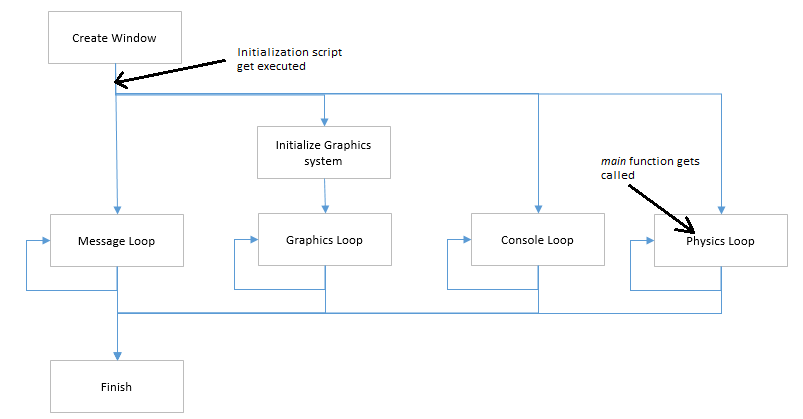
\includegraphics[width=6in]{CycleIntercept.png}
				\caption{Flow cycle of the simulation.}
				\label{figure:CycleIntercept}
			\end{figure}
		\end{minipage}
	\end{center}
\vspace{0.5cm}
The following is an example of a main function that prints a temperature to the interactive window and allows the heat input to be increased using the \textit{A} and \textit{Z} key presses:
\newline
\noindent
\begin{lstlisting}{style=myLuastyle}
chiThermoflowProcessInput("CHI_RESOURCES/Worlds/Tut02Heatblock/Input.txt");
chiThermoflowInitialize();

power=31.673e6;
AkeyDn=false;
ZkeyDn=false;
function main()
    chiThermoflowHBPerformTimeStep(0.0166667);
    cladT     =chiThermoflowGetHBProperty("Node_Temperature","h101",0);
    centerT   =chiThermoflowGetHBProperty("Node_Temperature","h101",10);

    if (WM_KEYDN.occured) then
       if (WM_KEYDN.iPar0 == 65) then AkeyDn = true; end
       if (WM_KEYDN.iPar0 == 90) then ZkeyDn = true; end
    end
    
    if (WM_KEYUP.occured or WM_MOUSELEAVE.occured) then
       if (WM_KEYUP.iPar0 == 65) then AkeyDn = false; end
       if (WM_KEYUP.iPar0 == 90) then ZkeyDn = false; end
    end
    
    if (AkeyDn) then power=power+1.0e6; end
    if (ZkeyDn) then power=power-1.0e6; end
    
    chiThermoflowSetHBProperty("HeatGeneration","h101",power);
    chiSetLabel("Tclad","Tclad ="..string.format("%5.3f", cladT),5,100);
    chiSetLabel("Tcent","Tcent ="..string.format("%5.3f", centerT),5,120);
    chiSetLabel("Heat" ,"Heat  ="..string.format("%5.3e", power),5,140);
end
\end{lstlisting}
\vspace{0.3cm}
\noindent
The output of the above script will resemble the following:
\noindent
	\begin{center}
		\begin{minipage}[c]{0.85\textwidth}
	
			\begin{figure}[H]
			
				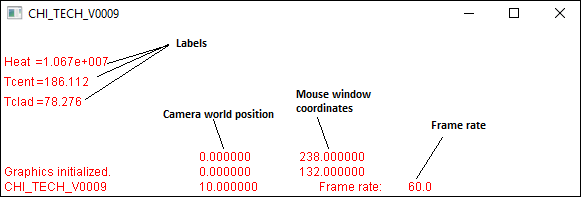
\includegraphics[width=6in]{Interactive.png}
				\caption{Interactive display.}
				\label{figure:Interactive}
			\end{figure}
		\end{minipage}
	\end{center}
\vspace{0.5cm}
%%
%%\newpage
%%\chead{References}
%%\begin{thebibliography}{1}

	
%%\end{thebibliography}





\end{document}